\documentclass{standalone}
\usepackage{tikz}

\begin{document}
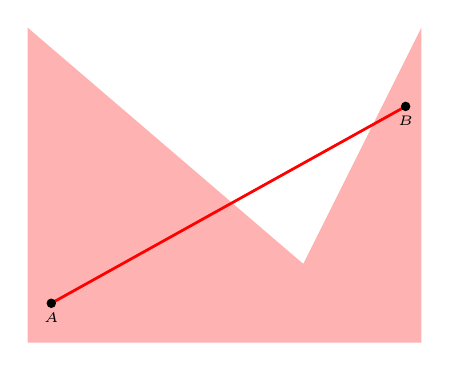
\begin{tikzpicture}
\coordinate (a) at (0,0);
\coordinate (b) at (0,4);
\coordinate (c) at (3.5,1);
\coordinate (d) at (5,4);
\coordinate (e) at (5,0);

\coordinate (A) at (.3,.5);
\coordinate (B) at (4.8,3);


\fill[red!30] (a) -- (b) -- (c) -- (d) -- (e); 

\draw[line width=1pt, red] (A) -- (B);
\draw[fill] (A) circle (1.5pt) node[below] {\tiny$A$};
\draw[fill] (B) circle (1.5pt) node[below] {\tiny$B$};
\end{tikzpicture}


\end{document}